\documentclass[a4paper,11pt]{article}

% ---------------------------------------------------------------------------
% Revision notes: Introduction to Statistics
% Compiled from the unit-wise lecture notes.
% Figures are generated by make-figures.R and live in figures/.
% ---------------------------------------------------------------------------

\usepackage[T1]{fontenc}
\usepackage{palatino}
\usepackage[english]{babel}
\usepackage[margin=25mm]{geometry}
\usepackage{amsmath, amssymb, mathtools}
\usepackage{graphicx}
\usepackage{float}
\usepackage{enumitem}
\usepackage{booktabs}
\usepackage{array}
\usepackage{xcolor}
\usepackage[most]{tcolorbox}
\usepackage{listings}
\usepackage{titlesec}
\usepackage[colorlinks=true, linkcolor=NavyBlue, urlcolor=NavyBlue]{hyperref}

\definecolor{NavyBlue}{HTML}{2B6CB0}
\definecolor{Warm}{HTML}{C05621}
\definecolor{Ink}{HTML}{1F2933}
\definecolor{PaleBlue}{HTML}{EBF4FB}
\definecolor{PaleGrey}{HTML}{F4F5F7}

\setlength{\parindent}{0pt}
\setlength{\parskip}{0.65em}

%% Let a float take more of a page before LaTeX defers it, and allow more
%% floats per page. Without this the figure-heavy sections leave large gaps.
\renewcommand{\topfraction}{0.9}
\renewcommand{\bottomfraction}{0.8}
\renewcommand{\textfraction}{0.07}
\renewcommand{\floatpagefraction}{0.75}

\titleformat{\section}{\Large\bfseries\color{Ink}}{\thesection}{0.7em}{}
\titleformat{\subsection}{\large\bfseries\color{Ink}}{\thesubsection}{0.7em}{}

% ---------------------------------------------------------------------------
% Boxes
% ---------------------------------------------------------------------------
\newtcolorbox{keybox}[1][]{
  colback=PaleBlue, colframe=NavyBlue, boxrule=0.4pt, arc=2pt,
  left=8pt, right=8pt, top=6pt, bottom=6pt,
  before upper={\setlength{\parskip}{0.6em}}, #1}

\newtcolorbox{watchbox}[1][]{
  colback=white, colframe=Warm, boxrule=0.8pt, arc=0pt,
  leftrule=3pt, rightrule=0pt, toprule=0pt, bottomrule=0pt,
  left=8pt, right=4pt, top=4pt, bottom=4pt,
  before upper={\setlength{\parskip}{0.6em}}, #1}

\newtcolorbox[auto counter, number within=section]{example}[1][]{
  colback=white, colframe=Ink!25, boxrule=0.4pt, arc=2pt,
  left=8pt, right=8pt, top=6pt, bottom=6pt,
  title={\normalfont\bfseries\color{Ink} Example \thetcbcounter},
  coltitle=Ink, colbacktitle=PaleGrey,
  before upper={\setlength{\parskip}{0.6em}}, #1}

\lstset{
  basicstyle=\ttfamily\small\color{Ink},
  backgroundcolor=\color{PaleGrey},
  frame=leftline, framerule=2pt, rulecolor=\color{NavyBlue},
  framexleftmargin=6pt, xleftmargin=8pt,
  breaklines=true, showstringspaces=false, aboveskip=10pt, belowskip=6pt}

\newcommand{\Rc}{\textbf{\color{NavyBlue}In R:}\ }

% ---------------------------------------------------------------------------
\title{\vspace{-1.5cm}\textbf{Introduction to Statistics}\\[0.2cm]
       \large A Revision of Basic Concepts}
\author{Kedar Kulkarni}
\date{\today}

\begin{document}
\maketitle

\vspace{-0.8cm}

\begin{keybox}
These notes revise the concepts covered in the course, in the order they were
taught. Each section states the idea, gives the formula, and works through one
or two examples. They are meant for revision, not as a replacement for the
lecture notes: the arguments here are compressed, and the detail is in the
originals.

Every figure is generated by the R script that accompanies these notes, so you
can reproduce or modify any of them.
\end{keybox}

\tableofcontents
\newpage

% ===========================================================================
\clearpage
\part*{Part I \quad Describing Data}
\addcontentsline{toc}{section}{\textbf{Part I \quad Describing Data}}
% ===========================================================================

Before we can reason about uncertainty, we need ways to describe what we have
observed. A dataset of a thousand numbers is not something anyone can hold in
their head. Descriptive statistics reduce it to a few numbers that capture where
the data sit, how spread out they are, and how two variables move together.

\section{Measures of Central Tendency}

A measure of central tendency answers a single question: \emph{if I had to
summarise this entire dataset with one number, what would it be?} There are
three standard answers, and they do not always agree.

\begin{keybox}
For a sample $x_1, x_2, \ldots, x_n$:

\textbf{Mean} --- the arithmetic average,
\[ \bar{x} = \frac{1}{n}\sum_{i=1}^{n} x_i \]

\textbf{Median} --- the middle value once the data are sorted. With $n$ odd it
is the $\frac{n+1}{2}$-th value; with $n$ even it is the average of the
$\frac{n}{2}$-th and $\left(\frac{n}{2}+1\right)$-th values.

\textbf{Mode} --- the value that occurs most often. A dataset may have no mode,
one mode, or several.
\end{keybox}

\subsection*{Which one to use}

The three coincide when the data are symmetric. When the data are skewed they
separate, and the order in which they separate is informative.

\begin{figure}[htbp]
\centering
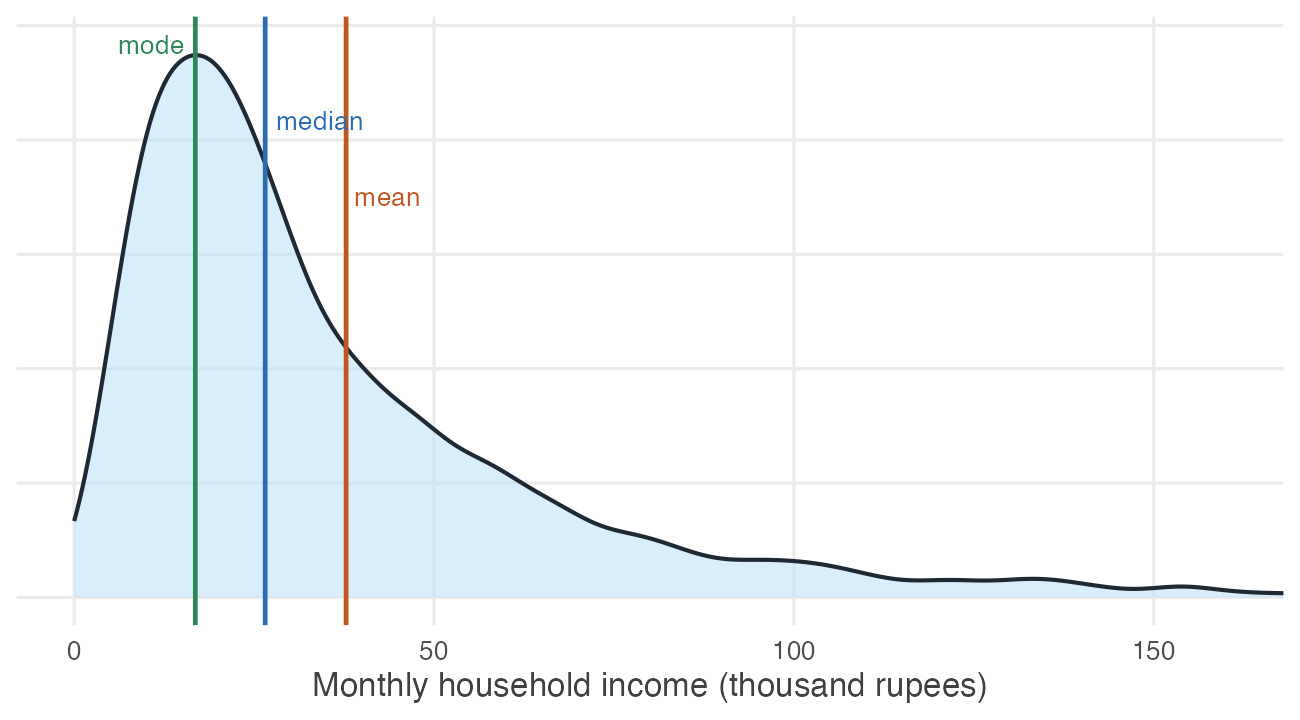
\includegraphics[width=0.85\textwidth]{figures/central-tendency.png}
\caption{Monthly household income, a right-skewed variable. A small number of
very high incomes pull the mean above the median, and the median above the mode.
For income data the median is usually the more honest summary --- it is the
income of the household in the middle, and it does not move when one billionaire
joins the sample.}
\end{figure}

\begin{watchbox}
\textbf{The mean is sensitive to extreme values; the median is not.}

This is why we report median household income, median wage and median house
price rather than their means. It is also why an average can be technically
correct and completely misleading.
\end{watchbox}

\begin{example}[label=ex:central]
The total number of road accidents recorded in Bengaluru in each month of 2023
was:
\[ 6,\; 13,\; 5,\; 7,\; 7,\; 3,\; 7,\; 2,\; 5,\; 6,\; 9,\; 8 \]
Find the mean, median and mode.

\medskip
\textbf{Solution.} Sorting the data first:
\[ 2,\; 3,\; 5,\; 5,\; 6,\; 6,\; 7,\; 7,\; 7,\; 8,\; 9,\; 13 \]

\emph{Mean.} $\bar{x} = \dfrac{78}{12} = 6.5$ accidents per month.

\emph{Median.} With $n = 12$ (even), average the 6th and 7th values:
$\dfrac{6+7}{2} = 6.5$.

\emph{Mode.} The value 7 appears three times, more than any other. The mode
is 7.

Here all three are close together, which tells us the data are roughly
symmetric --- there is no month so extreme that it distorts the average.
\end{example}

\Rc
\begin{lstlisting}
accidents <- c(6, 13, 5, 7, 7, 3, 7, 2, 5, 6, 9, 8)

mean(accidents)     # 6.5
median(accidents)   # 6.5
table(accidents)    # read off the most frequent value: 7
\end{lstlisting}

R has no built-in \texttt{mode()} for this purpose --- \texttt{mode()} reports
the storage type of an object, which is a different thing entirely. Use
\texttt{table()} and read off the largest count.

\section{Measures of Dispersion}

Two datasets can have the same mean and look nothing alike. Central tendency
tells us where the data sit; dispersion tells us how tightly they cluster there.

\begin{figure}[htbp]
\centering
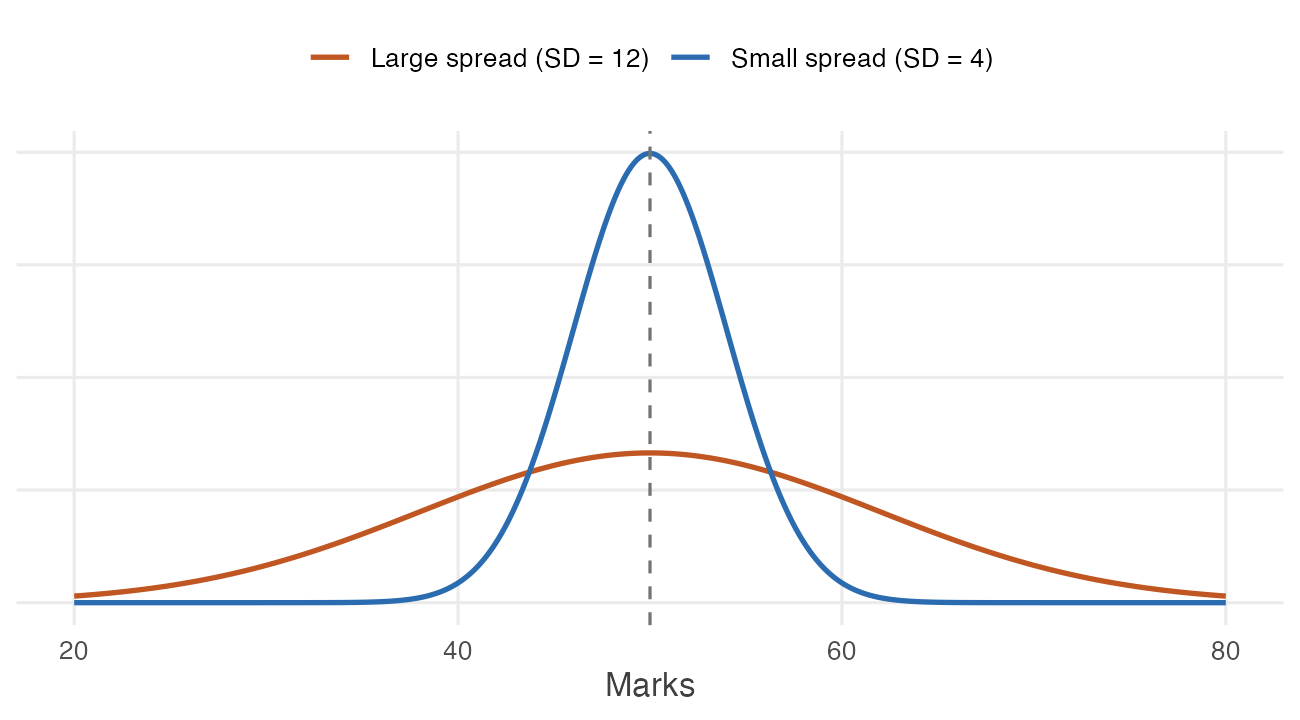
\includegraphics[width=0.8\textwidth]{figures/dispersion.png}
\caption{Two sets of marks with the same mean of 50. Knowing only the average
would tell you nothing about the difference between them --- and the difference
matters enormously to a student wondering whether 60 is an unremarkable score or
an excellent one.}
\end{figure}

\begin{keybox}
\textbf{Range} $=$ largest value $-$ smallest value. Simple, and almost
useless: it depends on only two observations.

\textbf{Sample variance}
\[ s^2 = \frac{1}{n-1}\sum_{i=1}^{n}(x_i - \bar{x})^2 \]

\textbf{Sample standard deviation} $s = \sqrt{s^2}$, which returns the measure
to the original units.

\textbf{Percentiles.} The $p$-th percentile is the value below which $p$ per
cent of the data lie. The 50th percentile is the median.
\end{keybox}

\subsection*{Why $n-1$ and not $n$?}

The deviations $x_i - \bar{x}$ are computed around the \emph{sample} mean rather
than the population mean, and the sample mean is by construction the value that
makes those squared deviations as small as possible. Dividing by $n$ would
therefore systematically underestimate the population variance. Dividing by
$n-1$ corrects for this.

\begin{example}
For the accident data above, find the standard deviation and the 80th
percentile.

\medskip
\textbf{Solution.} We know $\bar{x} = 6.5$. Squaring each deviation:
\begin{align*}
\sum (x_i - \bar{x})^2 &= (-0.5)^2 + (6.5)^2 + (-1.5)^2 + (0.5)^2 + (0.5)^2 + (-3.5)^2 \\
&\quad + (0.5)^2 + (-4.5)^2 + (-1.5)^2 + (-0.5)^2 + (2.5)^2 + (1.5)^2 \\
&= 89
\end{align*}

\[ s^2 = \frac{89}{11} = 8.09, \qquad s = \sqrt{8.09} = 2.84 \]

\emph{80th percentile.} $0.80 \times 12 = 9.6$, which is not an integer, so we
round up and take the 10th smallest value. From the sorted list that is
\textbf{8} accidents.

So in a typical month Bengaluru records about 6.5 accidents, give or take 2.8;
and in the worst two months of the year, at least 8.
\end{example}

\Rc
\begin{lstlisting}
sd(accidents)                  # 2.844
var(accidents)                 # 8.091
quantile(accidents, 0.80)      # 80th percentile
\end{lstlisting}

\begin{watchbox}
\texttt{quantile()} interpolates between observations by default, so it may
return a value that is not in the dataset. The hand method above --- round up
and take that observation --- is one of several defensible conventions. Both are
correct; they answer slightly different questions.
\end{watchbox}

\section{Scatter Plots and Correlation}

Everything so far has described one variable. Most interesting questions involve
two: does income rise with education? Do students who attend more classes score
higher?

The first step is always to plot the data. A \textbf{scatter plot} puts one
variable on each axis and a dot at each observation.

\begin{keybox}
The \textbf{correlation coefficient} $r$ measures the strength and direction of
the \emph{linear} association between two variables:
\[ r = \frac{\sum (x_i - \bar{x})(y_i - \bar{y})}
            {\sqrt{\sum (x_i - \bar{x})^2}\sqrt{\sum (y_i - \bar{y})^2}} \]

It always lies between $-1$ and $+1$.
\end{keybox}

\begin{figure}[htbp]
\centering
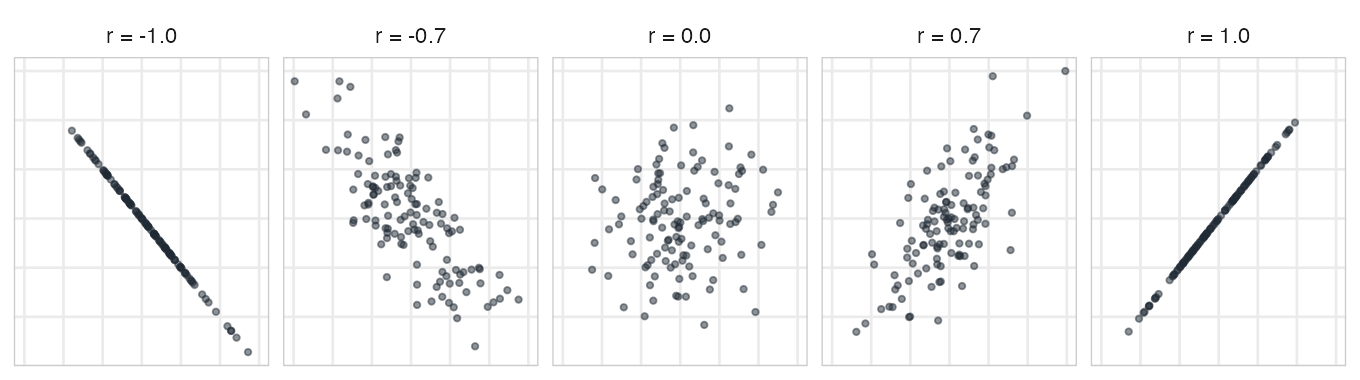
\includegraphics[width=\textwidth]{figures/correlation-strengths.png}
\caption{The same idea at five strengths. At $r = \pm 1$ the points lie exactly
on a line. At $r = 0$ there is no linear association. The sign tells you the
direction; the magnitude tells you how tightly the points hug the line.}
\end{figure}

\begin{table}[H]
\centering
\begin{tabular}{@{}lll@{}}
\toprule
\textbf{Value of $r$} & \textbf{Direction} & \textbf{Strength} \\
\midrule
$r = 0$          & None     & No linear association \\
$r = +1$         & Positive & Perfect \\
$r = -1$         & Negative & Perfect \\
$0 < r < +1$     & Positive & Closer to 1 is stronger \\
$-1 < r < 0$     & Negative & Closer to $-1$ is stronger \\
\bottomrule
\end{tabular}
\caption{Interpreting the correlation coefficient.}
\end{table}

\begin{figure}[htbp]
\centering
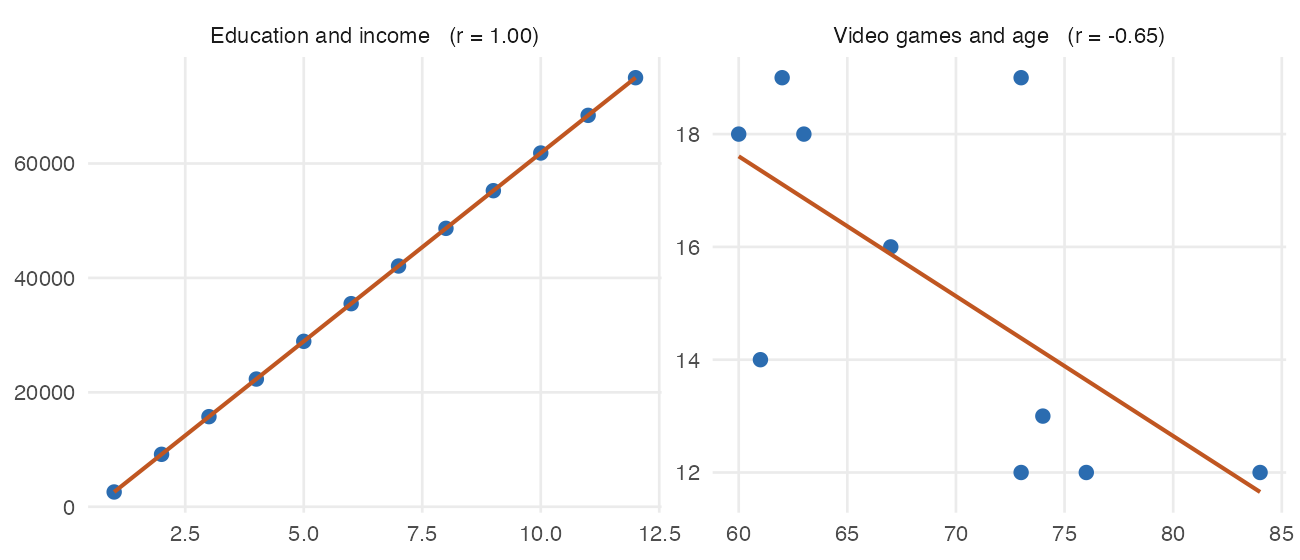
\includegraphics[width=\textwidth]{figures/scatter-examples.png}
\caption{Left: income against years of education, an almost perfect positive
association. Right: age against video games played per year, a moderate negative
association --- older teenagers play fewer games.}
\end{figure}

\begin{example}
The table records attendance and CGPA for six students.

\begin{center}
\begin{tabular}{@{}lcccccc@{}}
\toprule
Attendance & 20 & 25 & 30 & 35 & 40 & 45 \\
Grade      & 7.09 & 7.85 & 7.97 & 8.12 & 8.73 & 9.21 \\
\bottomrule
\end{tabular}
\end{center}

Find and interpret the correlation coefficient.

\medskip
\textbf{Solution.} Computing $r$ from the formula gives $r = 0.97$.

This is a strong positive association: students who attend more classes tend to
have higher grades, and the relationship is close to linear over the range
observed.
\end{example}

\begin{watchbox}
\textbf{Correlation is not causation, and $r$ only sees straight lines.}

A correlation of $0.97$ between attendance and grades does not establish that
attending causes higher grades --- more able or more motivated students may
simply do both. And a variable can be perfectly \emph{predictable} from another
while having $r = 0$, if the relationship is curved. Always look at the scatter
plot; never report $r$ without having seen one.
\end{watchbox}

\Rc
\begin{lstlisting}
attendance <- c(20, 25, 30, 35, 40, 45)
grade      <- c(7.09, 7.85, 7.97, 8.12, 8.73, 9.21)

plot(attendance, grade)                 # always plot first
cor(attendance, grade)                  # 0.9729
cor.test(attendance, grade)             # with a p-value and interval
\end{lstlisting}

% ===========================================================================
\clearpage
\part*{Part II \quad Probability}
\addcontentsline{toc}{section}{\textbf{Part II \quad Probability}}
% ===========================================================================

Descriptive statistics summarise the sample we have. But we almost never care
about the sample for its own sake --- we care about the population it came from,
and which particular sample we ended up with is a matter of chance. Probability
is the language for reasoning about that chance.

\section{Sample Space and Events}

\begin{keybox}
An \textbf{experiment} is any process whose outcome is uncertain but whose
possible outcomes are known.

The \textbf{sample space} $S$ is the set of all possible outcomes.

An \textbf{event} $A$ is any subset of the sample space, $A \subseteq S$.

If all outcomes are equally likely,
\[ P(A) = \frac{\text{number of outcomes in } A}{\text{number of outcomes in } S} \]
\end{keybox}

Because events are sets, the operations of set theory apply directly:

\begin{itemize}[leftmargin=1.4em, itemsep=2pt]
\item $A \cup B$ --- \emph{union}: the outcome is in $A$ \textbf{or} in $B$ (or both).
\item $A \cap B$ --- \emph{intersection}: the outcome is in $A$ \textbf{and} in $B$.
\item $A'$ (or $A^c$) --- \emph{complement}: the outcome is \textbf{not} in $A$.
\item De Morgan's laws: $(A \cup B)' = A' \cap B'$ and $(A \cap B)' = A' \cup B'$.
\end{itemize}

\begin{example}
A box contains three balls --- one red, one blue, one yellow. A ball is drawn,
replaced, and a second ball is drawn. Write down the sample space, the event
that the first ball is yellow, and the event that the same ball is drawn twice.

\medskip
\textbf{Solution.} Since the first ball is replaced, each draw has three
possibilities and the two draws are independent, giving $3 \times 3 = 9$
outcomes:
\[ S = \{(r,r), (r,b), (r,y), (b,r), (b,b), (b,y), (y,r), (y,b), (y,y)\} \]

First ball yellow: $A = \{(y,r), (y,b), (y,y)\}$, so $P(A) = 3/9 = 1/3$.

Same ball twice: $B = \{(r,r), (b,b), (y,y)\}$, so $P(B) = 3/9 = 1/3$.
\end{example}

\section{The Axioms of Probability}

\begin{keybox}
\textbf{1. Non-negativity.} $0 \le P(A) \le 1$ for every event $A$.

\textbf{2. Certainty.} $P(S) = 1$ --- something in the sample space must happen.

\textbf{3. Addition rule.} For any two events,
\[ P(A \cup B) = P(A) + P(B) - P(A \cap B) \]

Two consequences worth memorising:
\[ P(A') = 1 - P(A) \qquad\text{and}\qquad P(A \cap B') = P(A) - P(A \cap B) \]
\end{keybox}

\subsection*{Why subtract the intersection?}

Adding $P(A)$ and $P(B)$ counts every outcome in both events \emph{twice}.
Subtracting $P(A \cap B)$ removes the double count. If the events cannot occur
together the intersection is empty and the correction vanishes.

\begin{keybox}
Two events are \textbf{disjoint} (or mutually exclusive) if they cannot occur at
the same time. For disjoint events $P(A \cap B) = 0$, so the addition rule
simplifies to
\[ P(A \cup B) = P(A) + P(B) \]
\end{keybox}

\begin{example}
A company has bid for two construction projects. The probability of winning the
first is $0.6$, the second $0.4$, and both $0.2$. Find the probability that the
company wins (a) at least one contract, (b) the first but not the second,
(c) neither, (d) exactly one.

\medskip
\textbf{Solution.} Let $A$ = wins first, $B$ = wins second. We are given
$P(A) = 0.6$, $P(B) = 0.4$, $P(A \cap B) = 0.2$.

\emph{(a) At least one} is the union:
\[ P(A \cup B) = 0.6 + 0.4 - 0.2 = 0.8 \]

\emph{(b) First but not second:}
\[ P(A \cap B') = P(A) - P(A \cap B) = 0.6 - 0.2 = 0.4 \]

\emph{(c) Neither} is the complement of the union:
\[ P((A \cup B)') = 1 - 0.8 = 0.2 \]

\emph{(d) Exactly one} means first-not-second \emph{or} second-not-first. These
two are disjoint, so we may add them:
\[ 0.4 + \big(P(B) - P(A \cap B)\big) = 0.4 + 0.2 = 0.6 \]

Note that the company is more likely to win exactly one contract $(0.6)$ than to
win both $(0.2)$ or neither $(0.2)$ combined.
\end{example}

\section{Conditional Probability and Independence}

Often we learn something partway through. The probability that it rains today is
one thing; the probability that it rains \emph{given} that the sky is already
overcast is another. Conditional probability is how we update.

\begin{keybox}
The probability of $B$ \textbf{given} that $A$ has occurred is
\[ P(B \mid A) = \frac{P(A \cap B)}{P(A)}, \qquad P(A) > 0 \]

Rearranging gives the \textbf{multiplication rule}:
\[ P(A \cap B) = P(A)\,P(B \mid A) = P(B)\,P(A \mid B) \]
\end{keybox}

The intuition behind the formula is worth holding onto. Conditioning on $A$
throws away every outcome outside $A$, so $A$ becomes the new sample space. We
therefore count the outcomes in both $A$ and $B$, and divide by the outcomes in
$A$ rather than by the outcomes in $S$.

\begin{keybox}
Events $A$ and $B$ are \textbf{independent} if knowing one has occurred tells
you nothing about the other:
\[ P(B \mid A) = P(B) \quad\Longleftrightarrow\quad P(A \cap B) = P(A)P(B) \]
\end{keybox}

\begin{watchbox}
\textbf{Disjoint and independent are not the same thing --- they are close to
opposites.}

Disjoint asks: \emph{can both happen at once?} Independent asks: \emph{does one
happening change the chance of the other?}

If $A$ and $B$ are disjoint and $A$ occurs, then $B$ definitely has \emph{not}
occurred. That is about as far from "tells you nothing" as it is possible to
get. Two disjoint events with non-zero probability are always dependent.
\end{watchbox}

\begin{example}
Two people are chosen at random, without replacement, from a group of 4 women
and 6 men. Find the probability that (a) both are women, (b) one is a woman and
the other a man.

\medskip
\textbf{Solution.} Let $W_1$ be the event that the first person is a woman, and
$W_2$ that the second is.

\emph{(a)} The first draw: $P(W_1) = \frac{4}{10}$. Given that a woman was drawn
first, 3 women remain among 9 people, so $P(W_2 \mid W_1) = \frac{3}{9}$.
\[ P(W_1 \cap W_2) = \frac{4}{10} \times \frac{3}{9} = \frac{12}{90} = \frac{2}{15} \]

\emph{(b)} One of each can happen two ways --- man then woman, or woman then
man --- and these are disjoint, so we add:
\[ \frac{6}{10}\times\frac{4}{9} \;+\; \frac{4}{10}\times\frac{6}{9}
   \;=\; \frac{24}{90} + \frac{24}{90} \;=\; \frac{8}{15} \]

Because the sampling is \emph{without replacement}, the draws are not
independent: $P(W_2 \mid W_1) = \frac{3}{9}$, which is not $P(W_2)$. Had the
first person been put back, the two draws would have been independent and the
first answer would have been $\frac{4}{10}\times\frac{4}{10}$.
\end{example}

\section{Bayes' Theorem}

Sometimes we know $P(B \mid A)$ but want $P(A \mid B)$ --- the conditional
probability in reverse. A test tells us the probability of a positive result
given the disease; what we actually want is the probability of the disease given
a positive result.

\begin{keybox}
\textbf{Law of total probability.} For any event $A$,
\[ P(B) = P(B \mid A)P(A) + P(B \mid A')P(A') \]
That is, the probability of $B$ is a weighted average of its conditional
probabilities, weighted by how likely each condition is.

\textbf{Bayes' theorem.}
\[ P(A \mid B) = \frac{P(A \cap B)}{P(B)}
              = \frac{P(B \mid A)P(A)}{P(B \mid A)P(A) + P(B \mid A')P(A')} \]
\end{keybox}

\begin{example}
An insurance company believes people are either accident-prone or not. An
accident-prone person has an accident in a year with probability $0.1$; for
everyone else the probability is $0.05$. Twenty per cent of new policyholders
are accident-prone.

(a) What is the probability that a new policyholder has an accident in the first
year? (b) Given that a new policyholder \emph{did} have an accident, what is the
probability that they are accident-prone?

\medskip
\textbf{Solution.} Let $H$ = accident-prone, $A$ = has an accident in year one.
We are given $P(H) = 0.2$, $P(A \mid H) = 0.1$, $P(A \mid H') = 0.05$.

\emph{(a)} By the law of total probability,
\[ P(A) = (0.1)(0.2) + (0.05)(0.8) = 0.02 + 0.04 = 0.06 \]
So 6 per cent of new policyholders have an accident in their first year.

\emph{(b)} By Bayes' theorem,
\[ P(H \mid A) = \frac{P(A \mid H)P(H)}{P(A)}
               = \frac{(0.1)(0.2)}{0.06} = \frac{1}{3} \]

Read the two numbers together. Before observing anything, a new policyholder had
a $20\%$ chance of being accident-prone. After one accident that rises to
$33\%$. The accident is genuine evidence --- but it is far from proof, because
most accidents are had by the much larger group of ordinary drivers.
\end{example}

% ===========================================================================
\clearpage
\part*{Part III \quad Discrete Random Variables}
\addcontentsline{toc}{section}{\textbf{Part III \quad Discrete Random Variables}}
% ===========================================================================

\section{Random Variables and the Probability Mass Function}

\begin{keybox}
A \textbf{random variable} $X$ assigns a number to each outcome of an
experiment. It is \textbf{discrete} if it can take only a countable number of
values.

The \textbf{probability mass function} (pmf) gives the probability of each value:
\[ f(x) = P(X = x) \]

Every pmf satisfies $f(x) \ge 0$ for all $x$, and $\sum_x f(x) = 1$.
\end{keybox}

The convention is that a capital letter $X$ names the random variable and the
lowercase $x$ denotes a particular value it might take.

\begin{figure}[htbp]
\centering
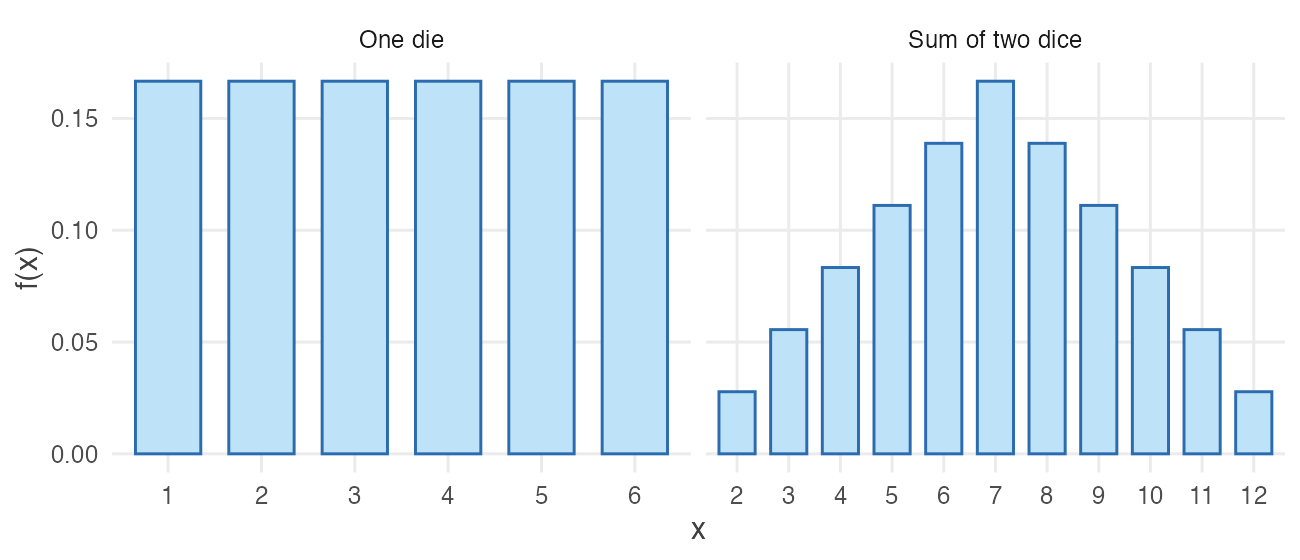
\includegraphics[width=\textwidth]{figures/pmf-dice.png}
\caption{Left: the pmf of a single fair die --- all six values equally likely.
Right: the pmf of the sum of two dice. The second is triangular rather than flat
because there are six ways to make a 7 and only one way to make a 2.}
\end{figure}

\begin{example}
A pair of fair dice is rolled and $X$ is their sum. Give the pmf.

\medskip
\textbf{Solution.} There are $6 \times 6 = 36$ equally likely outcomes. Counting
the ways of making each total:

\begin{center}
\begin{tabular}{@{}lccccccccccc@{}}
\toprule
$x$    & 2 & 3 & 4 & 5 & 6 & 7 & 8 & 9 & 10 & 11 & 12 \\
Ways   & 1 & 2 & 3 & 4 & 5 & 6 & 5 & 4 & 3 & 2 & 1 \\
$f(x)$ & $\frac{1}{36}$ & $\frac{2}{36}$ & $\frac{3}{36}$ & $\frac{4}{36}$
       & $\frac{5}{36}$ & $\frac{6}{36}$ & $\frac{5}{36}$ & $\frac{4}{36}$
       & $\frac{3}{36}$ & $\frac{2}{36}$ & $\frac{1}{36}$ \\
\bottomrule
\end{tabular}
\end{center}

The counts sum to 36, so the probabilities sum to 1, as any pmf must.
\end{example}

\section{Expectation and Variance}

\begin{keybox}
The \textbf{expected value} of a discrete random variable is the weighted
average of its possible values, weighted by their probabilities:
\[ E[X] = \mu = \sum_x x\, f(x) \]

The \textbf{variance} measures spread around that average:
\[ \mathrm{Var}[X] = \sigma^2 = E\big[(X-\mu)^2\big] = E[X^2] - \big(E[X]\big)^2 \]

The second form is almost always the easier one to compute.
\end{keybox}

Expectation is a \emph{long-run} average, not a prediction. The expected value
of a single die is 3.5, a value the die can never show. What it means is that if
you roll many times and average the results, you will land near 3.5.

\begin{keybox}
\textbf{Useful properties.} For a constant $c$,
\[ E[cX] = c\,E[X], \qquad E[X + c] = E[X] + c \]
\[ \mathrm{Var}[cX] = c^2\,\mathrm{Var}[X], \qquad \mathrm{Var}[X + c] = \mathrm{Var}[X] \]

Adding a constant shifts the distribution without stretching it, so the variance
is unchanged. Multiplying stretches it, and the variance picks up the square.
\end{keybox}

\begin{example}
For the sum of two dice, find $E[X]$ and $\mathrm{Var}[X]$.

\medskip
\textbf{Solution.} Using the pmf from the previous example,
\[ E[X] = 2\cdot\tfrac{1}{36} + 3\cdot\tfrac{2}{36} + \cdots + 12\cdot\tfrac{1}{36} = 7 \]

For the variance we need $E[X^2]$:
\[ E[X^2] = 2^2\cdot\tfrac{1}{36} + 3^2\cdot\tfrac{2}{36} + \cdots + 12^2\cdot\tfrac{1}{36} = 54.83 \]
\[ \mathrm{Var}[X] = E[X^2] - (E[X])^2 = 54.83 - 49 = 5.83 \]

So $\sigma = \sqrt{5.83} = 2.42$. A typical roll gives a total within about 2.4
of 7.
\end{example}

\begin{example}
A lawyer may charge a fixed fee of Rs.~$2{,}000$, or take a
contingency fee of Rs.~$8{,}000$ if she wins and nothing if she
loses. She wins with probability $0.3$. Which has the higher expected value?

\medskip
\textbf{Solution.} The fixed fee involves no uncertainty: $E[X] = 2000$.

For the contingency fee,
\[ E[X] = 8000(0.3) + 0(0.7) = 2400 \]

The contingency fee is worth Rs.~$400$ more \emph{on average}. But
notice what the average hides: it pays nothing $70\%$ of the time. Expected value
alone is not enough to choose between them --- that depends on how much risk she
can absorb.
\end{example}

\section{The Binomial Distribution}

\begin{keybox}
$X$ is a \textbf{binomial} random variable, written $X \sim b(n, p)$, if all
four conditions hold:

\begin{enumerate}[leftmargin=1.6em, itemsep=1pt]
\item There is a \textbf{fixed} number of trials, $n$.
\item Each trial has only two outcomes, success and failure.
\item The trials are \textbf{independent}.
\item The probability of success $p$ is the \textbf{same} on every trial.
\end{enumerate}

$X$ counts the number of successes, and
\[ f(r) = P(X = r) = \binom{n}{r} p^{r}(1-p)^{n-r} \]
\[ E[X] = np, \qquad \mathrm{Var}[X] = np(1-p) \]
\end{keybox}

The formula has a readable structure: $p^r(1-p)^{n-r}$ is the probability of one
particular sequence with $r$ successes, and $\binom{n}{r}$ counts how many such
sequences there are.

\begin{figure}[htbp]
\centering
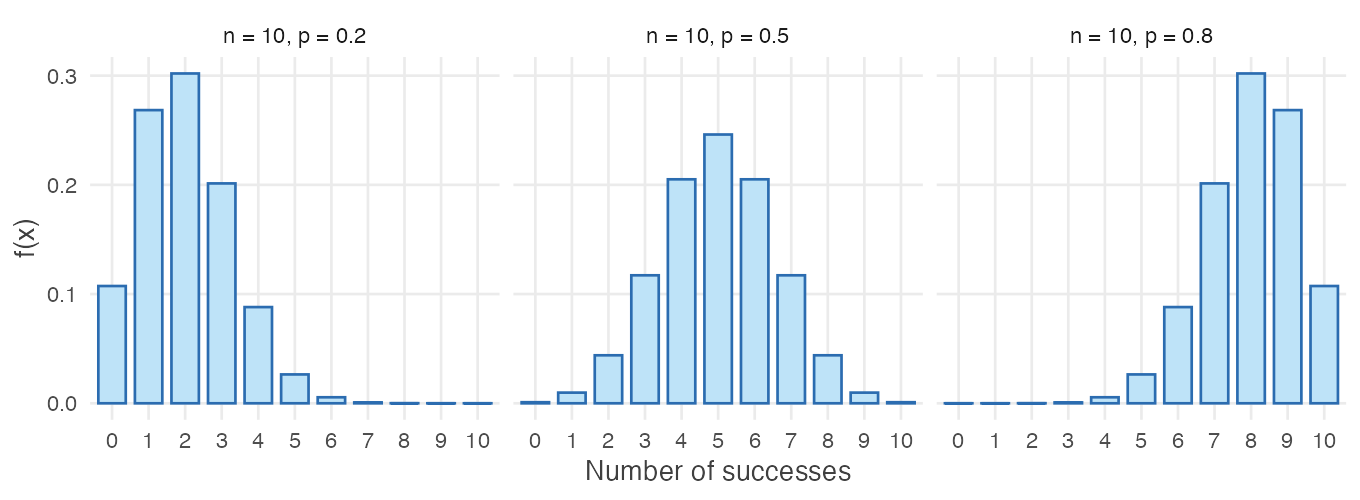
\includegraphics[width=\textwidth]{figures/binomial-pmf.png}
\caption{The binomial for three values of $p$, with $n$ fixed at 10. The
distribution is symmetric at $p = 0.5$ and skewed towards whichever outcome is
more likely otherwise.}
\end{figure}

\begin{watchbox}
Check the four conditions before using the formula. The most commonly violated
is the fourth. Sampling \emph{without replacement} from a small population
changes $p$ at each draw, and the variable is not binomial --- drawing 5 bulbs
from a box of 15 is not a binomial experiment.
\end{watchbox}

\begin{example}
Eighty per cent of Bengaluru start-ups turn a profit in their first year. In a
random sample of 20, what is the probability that exactly 7 do?

\medskip
\textbf{Solution.} Here $n = 20$, $p = 0.80$, $r = 7$.
\[ P(X = 7) = \binom{20}{7}(0.80)^{7}(0.20)^{13} = 0.0000133 \]

Vanishingly unlikely --- and it should be. We expect $np = 16$ profitable
start-ups, so 7 is nine below the mean.
\end{example}

\begin{example}
A fluorescent bulb burns for at least 500 hours with probability $0.90$. Of 8
bulbs, find the probability that (a) all 8 last that long, (b) exactly 7 do,
(c) at least 7 do. (d) What are the mean and variance?

\medskip
\textbf{Solution.} $n = 8$, $p = 0.90$.
\begin{align*}
P(X = 8) &= \binom{8}{8}(0.9)^8(0.1)^0 = 0.4305 \\
P(X = 7) &= \binom{8}{7}(0.9)^7(0.1)^1 = 0.3826 \\
P(X \ge 7) &= 0.4305 + 0.3826 = 0.8131
\end{align*}
\[ E[X] = np = 7.2, \qquad \mathrm{Var}[X] = np(1-p) = 8(0.9)(0.1) = 0.72 \]
\end{example}

\Rc
\begin{lstlisting}
dbinom(7, size = 20, prob = 0.80)     # P(X = 7) exactly
pbinom(6, size = 20, prob = 0.80)     # P(X <= 6) cumulative
1 - pbinom(6, size = 20, prob = 0.80) # P(X >= 7)
\end{lstlisting}

\begin{watchbox}
The argument is \texttt{prob}, not \texttt{probability}. Writing
\texttt{dbinom(7, size = 20, probability = 0.8)} returns an error, not a wrong
answer --- which at least fails loudly.

Use \texttt{d} for a single value and \texttt{p} for a cumulative probability.
\texttt{pbinom(6, 20, 0.8)} is far quicker than summing seven \texttt{dbinom}
calls.
\end{watchbox}

\section{The Poisson Distribution}

The binomial counts successes in a fixed number of trials. Sometimes there are
no trials to count --- we want the number of events in an interval of time or
space, where the events could in principle occur at any moment.

\begin{keybox}
$X$ is \textbf{Poisson} with rate $\lambda$ if it counts the number of events in
a fixed interval, occurring independently at a constant average rate:
\[ f(x) = P(X = x) = \frac{e^{-\lambda}\lambda^{x}}{x!}, \qquad x = 0, 1, 2, \ldots \]
\[ E[X] = \lambda, \qquad \mathrm{Var}[X] = \lambda \]
\end{keybox}

The mean and the variance are the same number. This is a strong and testable
claim about data: if a count variable has a variance much larger than its mean,
it is not Poisson.

Typical examples: typos on a page, cars through an intersection in a minute,
goals in a football match, customers at an ATM in ten minutes.

\begin{figure}[htbp]
\centering
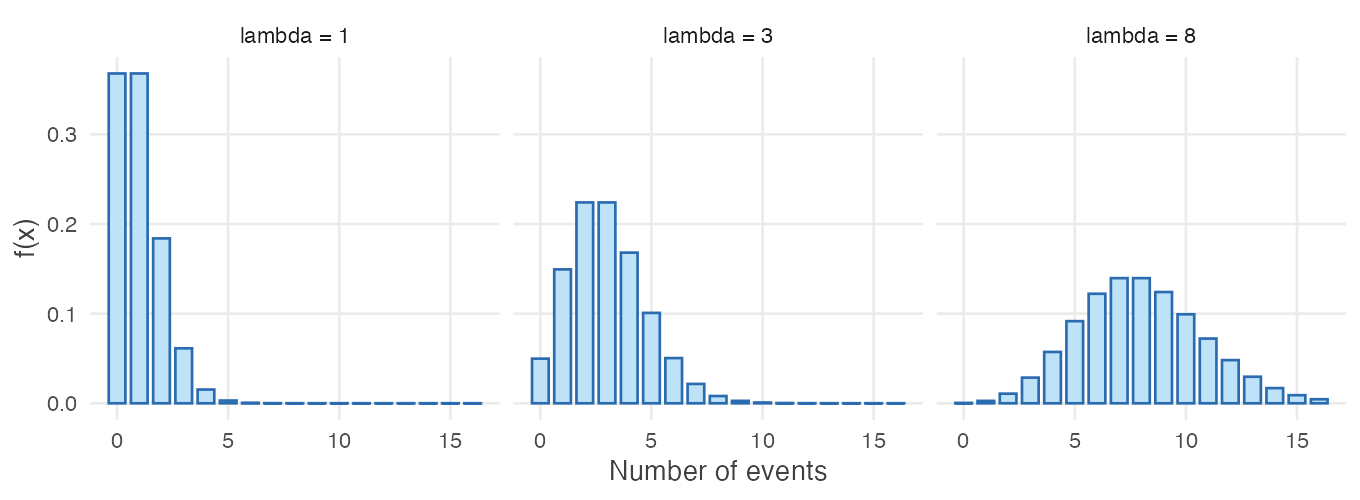
\includegraphics[width=\textwidth]{figures/poisson-pmf.png}
\caption{The Poisson at three rates. At small $\lambda$ the distribution is
bunched against zero and strongly skewed; as $\lambda$ grows it spreads out and
becomes more symmetric.}
\end{figure}

\begin{example}
A printed page has on average 3 typos. Find the probability that a page has
(a) at least one typo, (b) at most one typo.

\medskip
\textbf{Solution.} $\lambda = 3$.

\emph{(a)} Going through the complement is much less work than summing an
infinite series:
\[ P(X \ge 1) = 1 - P(X = 0) = 1 - \frac{e^{-3}3^{0}}{0!} = 1 - 0.0498 = 0.9502 \]

\emph{(b)}
\[ P(X \le 1) = P(X=0) + P(X=1) = 0.0498 + 0.1494 = 0.1991 \]
\end{example}

\begin{example}
On a day safari, tourists see on average 5 lions. What is the probability of
seeing fewer than four?

\medskip
\textbf{Solution.} $\lambda = 5$, and "fewer than four" means $0, 1, 2$ or $3$:
\[ P(X < 4) = \sum_{x=0}^{3}\frac{e^{-5}5^{x}}{x!} = 0.265 \]
\end{example}

\Rc
\begin{lstlisting}
dpois(0, lambda = 3)        # P(X = 0)
ppois(1, lambda = 3)        # P(X <= 1)
ppois(3, lambda = 5)        # P(X < 4), since X is a whole number
\end{lstlisting}

\section{The Negative Binomial Distribution}

The binomial fixes the number of trials and lets the number of successes vary.
The negative binomial does the reverse: it fixes the number of successes we are
waiting for and asks how many trials it takes.

\begin{keybox}
Let $X$ be the number of trials needed to obtain the $r$-th success, where each
trial succeeds independently with probability $p$. Then
\[ P(X = n) = \binom{n-1}{r-1}p^{r}(1-p)^{n-r}, \qquad n = r, r+1, \ldots \]
\[ E[X] = \frac{r}{p}, \qquad \mathrm{Var}[X] = \frac{r(1-p)}{p^{2}} \]
\end{keybox}

The binomial coefficient is $\binom{n-1}{r-1}$ rather than $\binom{n}{r}$
because the last trial is \emph{not} free to vary --- it must be a success, or
we would not have stopped there. The remaining $r-1$ successes may fall anywhere
among the first $n-1$ trials.

The expected value is worth remembering on its own: if a trial succeeds with
probability $p$, you should expect to wait $1/p$ trials for one success. At
$p = 0.2$ that is five attempts.

\begin{example}
An exploratory oil well strikes oil with probability $0.20$. What is the
probability that the first strike comes on the third well drilled?

\medskip
\textbf{Solution.} We want the $r = 1$st success on trial $n = 3$:
\[ P(X = 3) = \binom{2}{0}(0.2)^{1}(0.8)^{2} = 0.128 \]
\end{example}

\begin{example}
An insurance agent sells a policy to a household with probability $0.40$, and
needs 5 policies for promotion. What is the probability that the fifth sale
happens at the 11th household? If the oil company of the previous example wants
three producing wells, how many must it expect to drill?

\medskip
\textbf{Solution.} For the agent, $r = 5$, $p = 0.4$, $n = 11$:
\[ P(X = 11) = \binom{10}{4}(0.4)^{5}(0.6)^{6} = 0.1003 \]

For the oil company, $r = 3$ and $p = 0.2$:
\[ E[X] = \frac{3}{0.2} = 15 \text{ wells}, \qquad
   \mathrm{Var}[X] = \frac{3(0.8)}{0.2^{2}} = 60 \]

Fifteen wells expected, with a standard deviation of $\sqrt{60} = 7.7$ --- so
the outcome is highly variable, and budgeting for exactly 15 would be unwise.
\end{example}

\begin{watchbox}
R's \texttt{dnbinom()} counts \emph{failures before} the $r$-th success, not
total trials. If $X$ is the number of trials, ask R for \texttt{n - r}:

\begin{lstlisting}
dnbinom(3 - 1, size = 1, prob = 0.2)    # 0.128
dnbinom(11 - 5, size = 5, prob = 0.4)   # 0.1003
\end{lstlisting}
\end{watchbox}

% ===========================================================================
\clearpage
\part*{Part IV \quad Continuous Random Variables}
\addcontentsline{toc}{section}{\textbf{Part IV \quad Continuous Random Variables}}
% ===========================================================================

\section{From Mass to Density}

A discrete variable takes countably many values. A continuous variable --- a
weight, a duration, a rainfall total --- takes any value in an interval.

That difference has a startling consequence.

\begin{keybox}
For a continuous random variable, $P(X = x) = 0$ for \emph{every} value $x$.

Probability attaches to \emph{intervals}, not to points. The
\textbf{probability density function} $f(x)$ gives probabilities as areas:
\[ P(a \le X \le b) = \int_{a}^{b} f(x)\,dx \]
with $f(x) \ge 0$ everywhere and total area $\int_{-\infty}^{\infty} f(x)\,dx = 1$.
\end{keybox}

If you say your weight is 75 kg you do not mean exactly $75.000\ldots$ kg; you
mean somewhere in a small interval around 75. There are infinitely many possible
values and no single one of them can carry positive probability, or the total
would exceed 1.

\begin{watchbox}
Because the endpoints carry zero probability, the inequalities do not matter:
\[ P(a \le X \le b) = P(a < X < b) \]
This is true for continuous variables and \textbf{false} for discrete ones,
where $P(X \le 3)$ and $P(X < 3)$ differ by $P(X = 3)$.
\end{watchbox}

\begin{figure}[htbp]
\centering
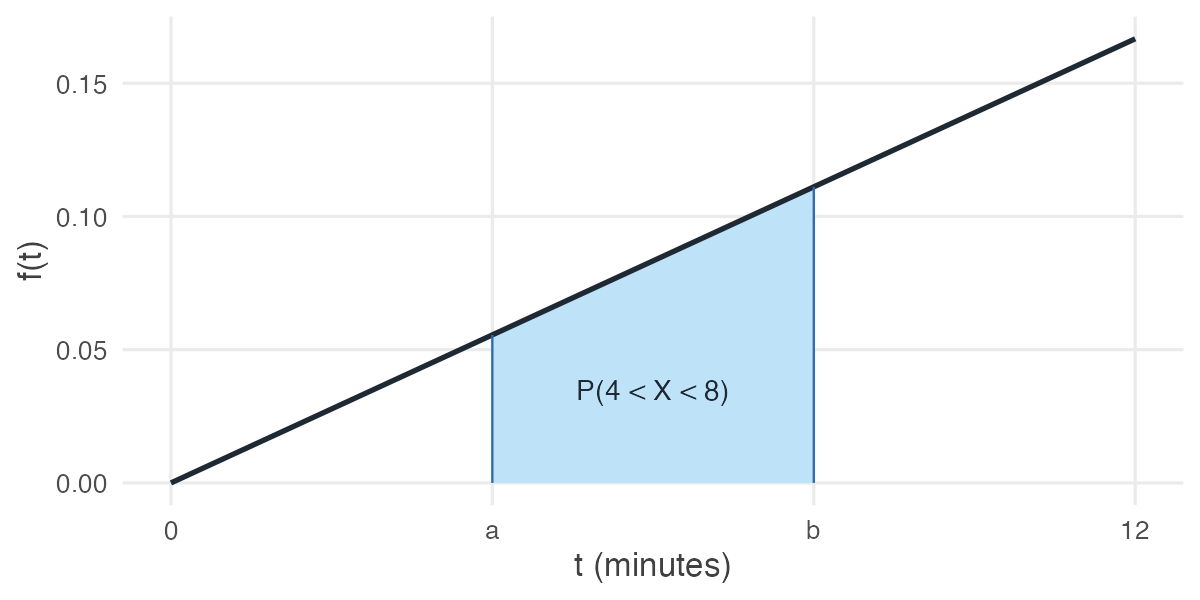
\includegraphics[width=0.75\textwidth]{figures/pdf-area.png}
\caption{A probability density function. The probability that $X$ falls between
$a$ and $b$ is the shaded area, obtained by integrating the density between
those limits. The total area under the curve is 1.}
\end{figure}

\begin{keybox}
Expectation and variance replace sums with integrals:
\[ E[X] = \int x\,f(x)\,dx, \qquad
   \mathrm{Var}[X] = \int x^{2} f(x)\,dx - \big(E[X]\big)^{2} \]
\end{keybox}

\begin{example}
Let $T$ be the length of a phone call in minutes, with density
\[ f(t) = \begin{cases} kt & 0 \le t \le 12 \\ 0 & \text{otherwise} \end{cases} \]
(a) Find $k$. (b) Find $P(T > 5)$. (c) Show that $E[T] = \mathrm{Var}[T]$.

\medskip
\textbf{Solution.}

\emph{(a)} The total area must be 1:
\[ \int_{0}^{12} kt\,dt = \left[\frac{kt^{2}}{2}\right]_{0}^{12}
 = \frac{144k}{2} = 72k = 1 \quad\Longrightarrow\quad k = \frac{1}{72} \]

\emph{(b)}
\[ P(T > 5) = 1 - \int_{0}^{5}\frac{t}{72}\,dt
 = 1 - \frac{1}{72}\left[\frac{t^{2}}{2}\right]_{0}^{5}
 = 1 - \frac{25}{144} = 0.826 \]

\emph{(c)}
\[ E[T] = \int_{0}^{12} t\cdot\frac{t}{72}\,dt
 = \frac{1}{72}\left[\frac{t^{3}}{3}\right]_{0}^{12} = \frac{1728}{216} = 8 \]
\[ E[T^{2}] = \int_{0}^{12} t^{2}\cdot\frac{t}{72}\,dt
 = \frac{1}{72}\left[\frac{t^{4}}{4}\right]_{0}^{12} = \frac{20736}{288} = 72 \]
\[ \mathrm{Var}[T] = 72 - 8^{2} = 8 \]

Both equal 8, though this is a coincidence of the particular density rather than
a general result.
\end{example}

\section{The Uniform Distribution}

The simplest continuous distribution: every value in an interval is as likely as
every other.

\begin{keybox}
$X \sim U(a,b)$ has constant density
\[ f(x) = \frac{1}{b-a}, \qquad a \le x \le b \]
\[ E[X] = \frac{a+b}{2}, \qquad \mathrm{Var}[X] = \frac{(b-a)^{2}}{12} \]
\end{keybox}

Because the density is flat, no integration is needed. Probability is just the
proportion of the interval covered:
\[ P(c \le X \le d) = \frac{d-c}{b-a} \]

\begin{figure}[htbp]
\centering
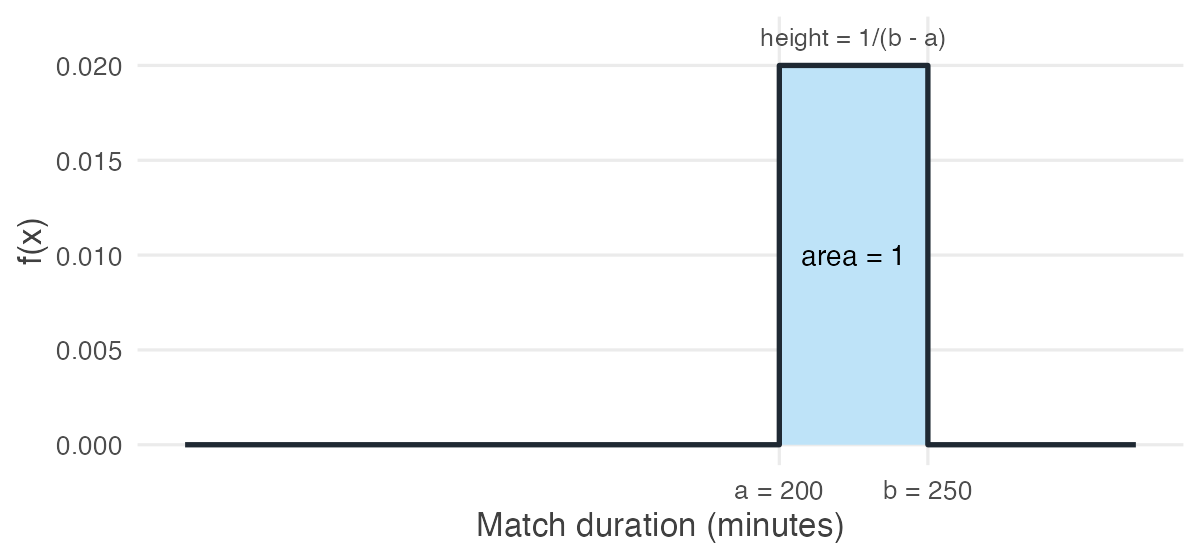
\includegraphics[width=0.72\textwidth]{figures/uniform.png}
\caption{The uniform density is a rectangle. Its height is $1/(b-a)$ precisely
so that height $\times$ base $= 1$, as every density must integrate to one.}
\end{figure}

\begin{example}
An IPL match lasts a uniformly distributed time between 200 and 250 minutes.
(a) Find the mean and standard deviation. (b) Find the probability a match lasts
between 220 and 240 minutes. (c) Find the 75th percentile.

\medskip
\textbf{Solution.} $X \sim U(200, 250)$, so $f(x) = 1/50$.

\emph{(a)}
\[ E[X] = \frac{200+250}{2} = 225 \text{ minutes}, \qquad
   \mathrm{Var}[X] = \frac{50^{2}}{12} = 208.33 \]
so $\sigma = 14.43$ minutes.

\emph{(b)}
\[ P(220 < X < 240) = \frac{240-220}{50} = 0.40 \]

\emph{(c)} We want the $x$ with $75\%$ of the area below it:
\[ \frac{x - 200}{50} = 0.75 \quad\Longrightarrow\quad x = 237.5 \text{ minutes} \]

So three matches in four finish within 237.5 minutes.
\end{example}

\section{The Normal Distribution}

The most important continuous distribution, and the one the rest of the course
depends on.

\begin{keybox}
$X \sim N(\mu, \sigma^{2})$ has density
\[ f(x) = \frac{1}{\sigma\sqrt{2\pi}}
   \exp\!\left(-\frac{1}{2}\frac{(x-\mu)^{2}}{\sigma^{2}}\right),
   \qquad -\infty < x < \infty \]
with $E[X] = \mu$ and $\mathrm{Var}[X] = \sigma^{2}$.
\end{keybox}

You will never need to integrate this by hand. What matters is its shape and the
role of its two parameters.

\begin{itemize}[leftmargin=1.4em, itemsep=2pt]
\item Bell-shaped and \textbf{symmetric} about $\mu$.
\item The mean, median and mode all coincide at $\mu$.
\item $\mu$ sets the \textbf{location}; $\sigma$ sets the \textbf{spread}.
\item Points of inflection at $\mu \pm \sigma$.
\item Total area 1; the curve never touches the horizontal axis.
\end{itemize}

\begin{figure}[htbp]
\centering
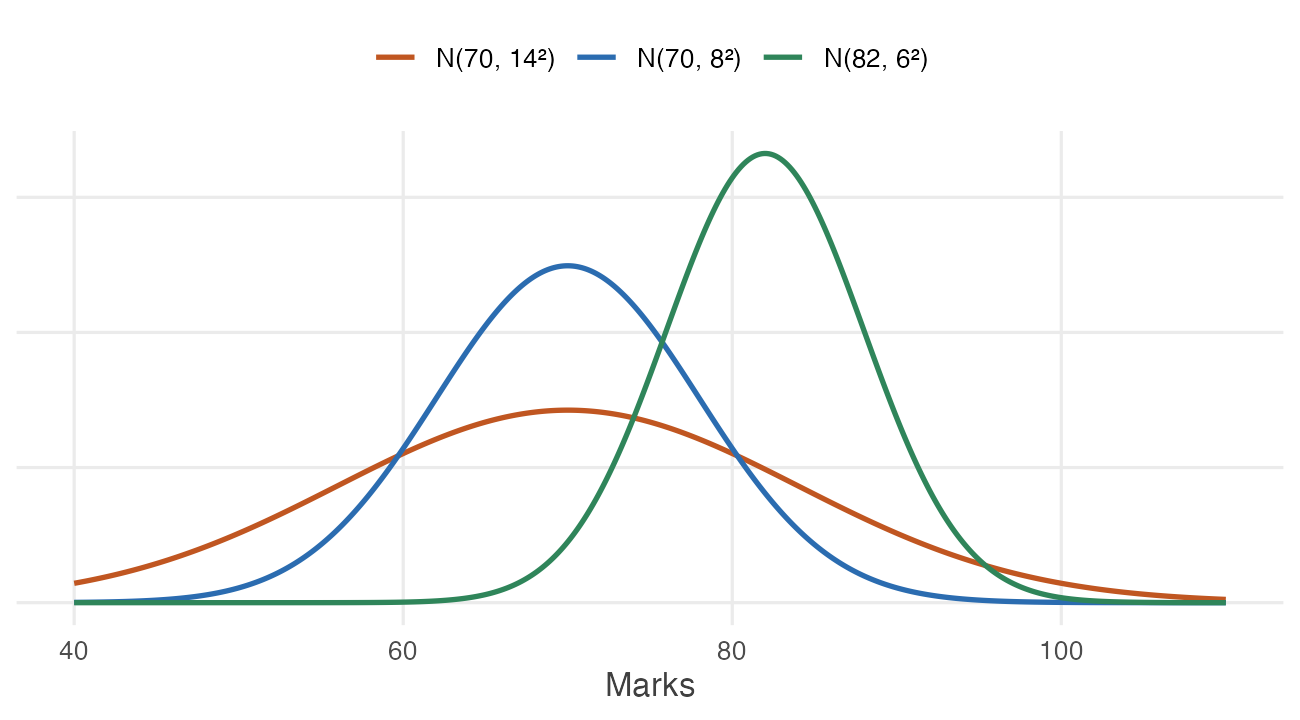
\includegraphics[width=0.85\textwidth]{figures/normal-shapes.png}
\caption{Changing $\mu$ slides the curve along the axis without altering its
shape; changing $\sigma$ makes it wider and flatter, or narrower and taller. The
area under each is 1, which is why a wider curve must also be shorter.}
\end{figure}

\subsection*{The empirical rule}

\begin{keybox}
For \emph{any} normal random variable, approximately
\begin{itemize}[leftmargin=1.4em, itemsep=1pt]
\item $68\%$ of values lie within $1$ standard deviation of the mean,
\item $95\%$ within $2$ standard deviations,
\item $99.7\%$ within $3$.
\end{itemize}
\end{keybox}

\begin{figure}[htbp]
\centering
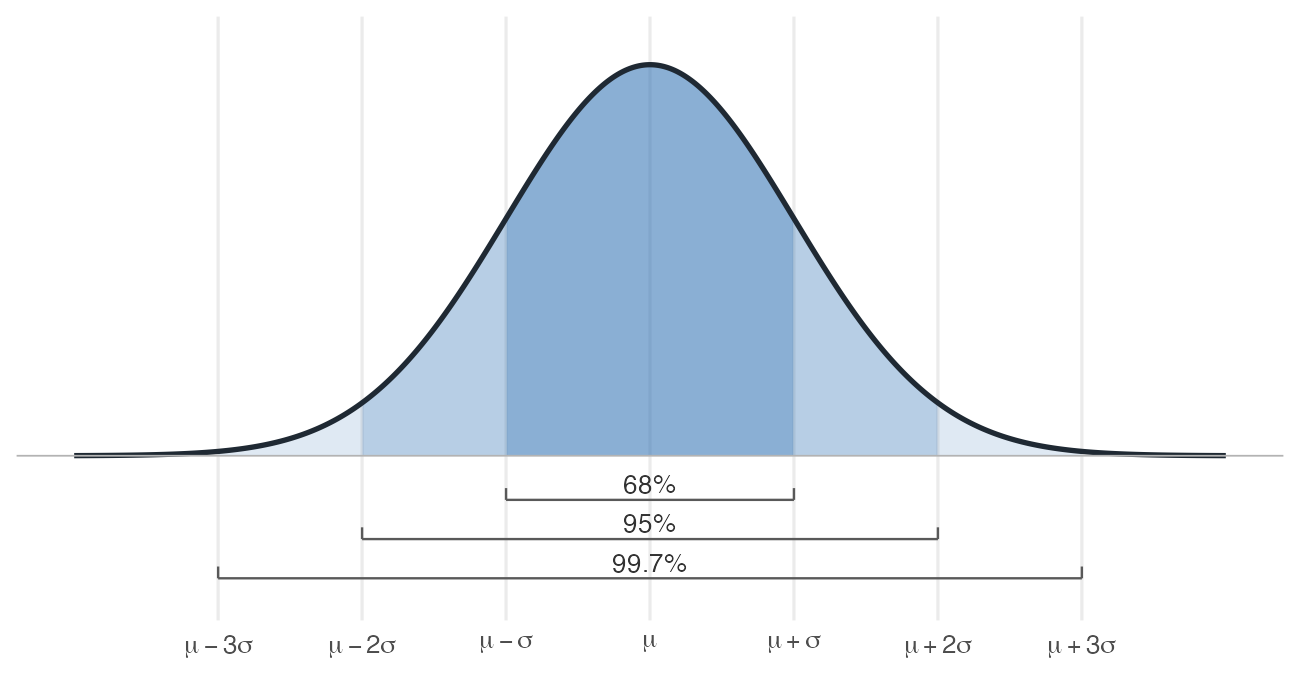
\includegraphics[width=0.85\textwidth]{figures/empirical-rule.png}
\caption{The 68--95--99.7 rule. Because the curve is symmetric, half of what
lies outside each band is in each tail --- so $2.5\%$ of values exceed
$\mu + 2\sigma$, and $16\%$ exceed $\mu + \sigma$.}
\end{figure}

The symmetry lets you answer most empirical-rule questions without a table. If
$95\%$ lies within $2\sigma$, then $5\%$ lies outside, split equally between the
two tails: $2.5\%$ above $\mu + 2\sigma$ and $2.5\%$ below $\mu - 2\sigma$.

\begin{example}
Heights in a population are normal with mean 173 cm and standard deviation 6 cm.
Approximate the proportion of people who are (a) shorter than 161 cm,
(b) taller than 179 cm, (c) between 161 and 185 cm.

\medskip
\textbf{Solution.} Express each bound as a distance from the mean in standard
deviations.

\emph{(a)} $161 = 173 - 12 = \mu - 2\sigma$. Below $\mu - 2\sigma$ lies half of
the $5\%$ outside the two-sigma band: $\mathbf{2.5\%}$.

\emph{(b)} $179 = 173 + 6 = \mu + \sigma$. Above $\mu + \sigma$ lies half of the
$32\%$ outside the one-sigma band: $\mathbf{16\%}$.

\emph{(c)} $161 = \mu - 2\sigma$ and $185 = \mu + 2\sigma$, so this is exactly
the two-sigma band: $\mathbf{95\%}$.
\end{example}

\section{The Standard Normal and $z$-Scores}

The empirical rule only answers questions at whole numbers of standard
deviations. For anything else we need a table --- and a table cannot be printed
for every possible $\mu$ and $\sigma$. The solution is to convert every normal
variable to a single common one.

\begin{keybox}
The \textbf{standard normal} $Z$ is normal with mean 0 and standard deviation 1,
written $Z \sim N(0,1)$.

Any normal variable can be \textbf{standardised}:
\[ Z = \frac{X - \mu}{\sigma} \]

The $z$-score says how many standard deviations $x$ lies from its mean. A
$z$ of $2$ means "two standard deviations above average", whatever the original
units were.
\end{keybox}

\begin{figure}[htbp]
\centering
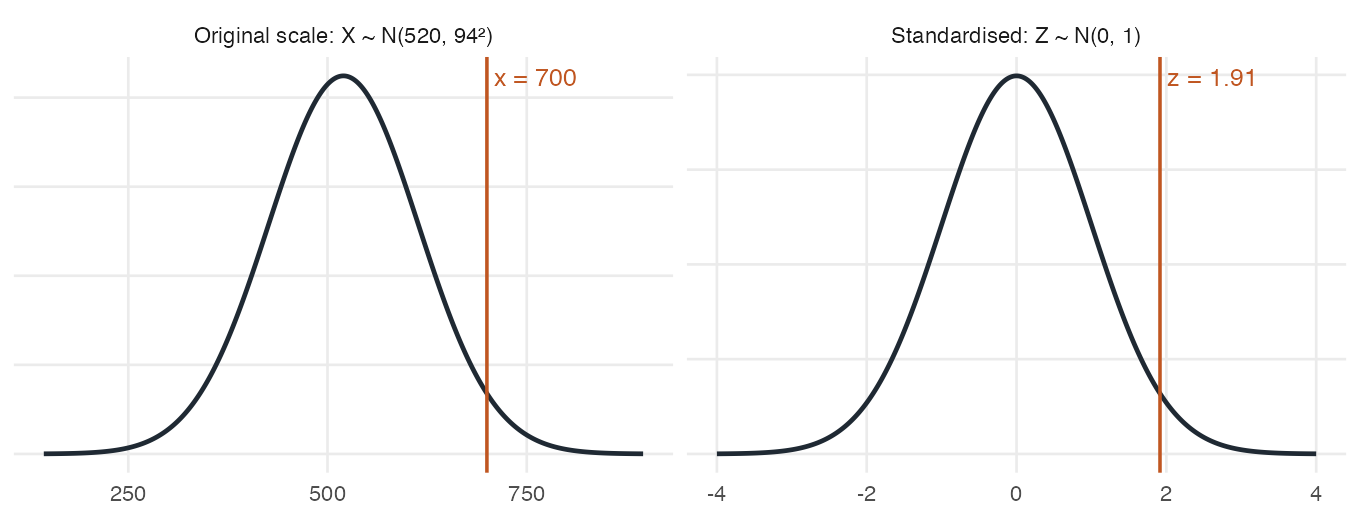
\includegraphics[width=\textwidth]{figures/standardising.png}
\caption{Standardising changes the numbers on the horizontal axis and nothing
else. A score of 700 on a test with mean 520 and standard deviation 94 becomes
$z = 1.91$; the shape of the curve, and the area to the right of the line, are
identical in both panels.}
\end{figure}

\subsection*{Reading the $Z$-table}

The table gives $P(Z < z)$ --- the area to the \emph{left} of $z$. To find
$P(Z < 1.22)$, look down the left column to $1.2$, across the top row to $0.02$,
and read off $0.8888$.

\begin{figure}[htbp]
\centering
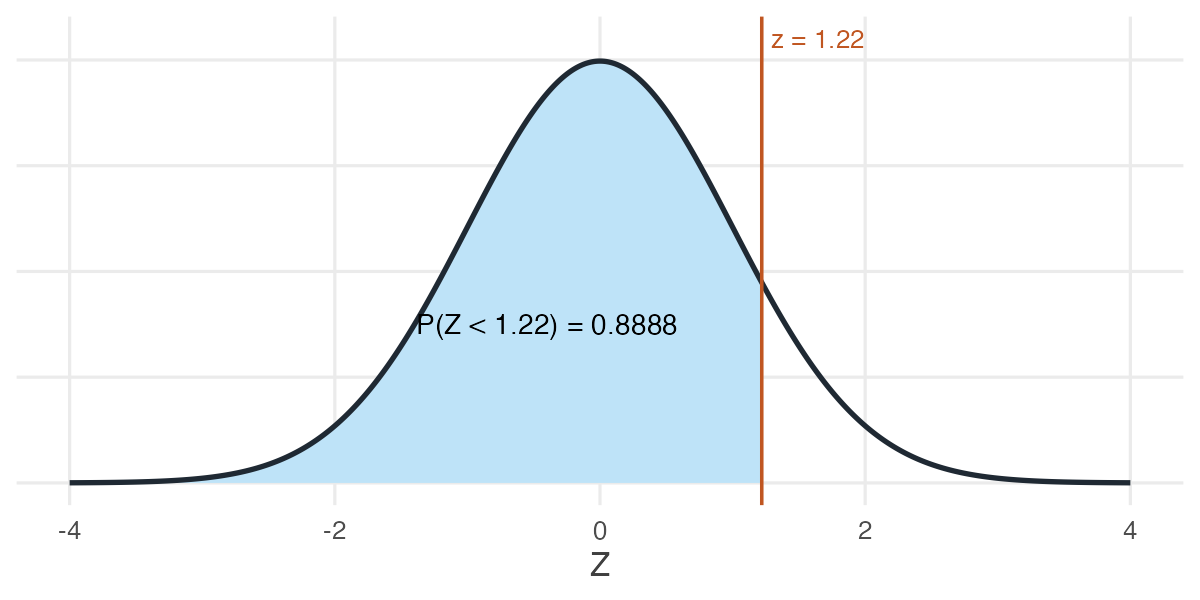
\includegraphics[width=0.72\textwidth]{figures/z-tail.png}
\caption{The table always reports the shaded area to the left. Every other
question is obtained from this one by subtraction.}
\end{figure}

\begin{keybox}
Three manipulations cover everything:
\[ P(Z > z) = 1 - P(Z < z) \]
\[ P(a < Z < b) = P(Z < b) - P(Z < a) \]
\[ P(Z < -z) = 1 - P(Z < z) \qquad\text{(by symmetry)} \]
\end{keybox}

\begin{watchbox}
A probability is never negative and never exceeds 1. If a $Z$-table calculation
produces $-0.236$, something has gone wrong --- most often a subtraction done in
the wrong order.
\end{watchbox}

\begin{example}
Scores on an achievement test are normal with mean 520 and standard deviation
94. Your score is 700. How many standard deviations above average is that, and
what percentage of candidates scored higher?

\medskip
\textbf{Solution.} Standardise:
\[ z = \frac{700 - 520}{94} = 1.91 \]
so the score is $1.91$ standard deviations above the mean.
\[ P(X > 700) = P(Z > 1.91) = 1 - P(Z < 1.91) = 1 - 0.9719 = 0.028 \]

Only about $2.8\%$ of candidates scored higher.
\end{example}

\subsection*{Working backwards: percentiles}

Sometimes the probability is given and the value is unknown --- a cutoff for the
top $10\%$, say. The table is then read in reverse.

\begin{keybox}
$z_{\alpha}$ is defined by $P(Z > z_{\alpha}) = \alpha$: the value with area
$\alpha$ to its \emph{right}.

To find the raw score, invert the standardising formula:
\[ x = \mu + z\sigma \]
\end{keybox}

\begin{example}
GRE quantitative scores are normal with mean 510 and standard deviation 92. What
score is needed to be in the top $10\%$?

\medskip
\textbf{Solution.} Top $10\%$ means $10\%$ of the area lies above, so $90\%$
lies below. From the table, the $z$ with $P(Z < z) = 0.90$ is $z = 1.28$.

Converting back to the original scale:
\[ x = \mu + z\sigma = 510 + 1.28(92) = 627.8 \]

A score of about \textbf{628} or higher is needed.
\end{example}

\Rc
\begin{lstlisting}
pnorm(1.22)                       # P(Z < 1.22) = 0.8888
1 - pnorm(700, mean = 520, sd = 94)   # P(X > 700), no standardising needed
qnorm(0.90)                       # the z with 90% below it: 1.2816
qnorm(0.90, mean = 510, sd = 92)  # the raw score directly: 627.9
\end{lstlisting}

\begin{keybox}
\textbf{\texttt{pnorm} goes from a value to a probability; \texttt{qnorm} goes
from a probability back to a value.}

Giving either function \texttt{mean} and \texttt{sd} lets it work on the
original scale, so R can skip the standardising step entirely. Standardising by
hand still matters --- it is what makes the $z$-score interpretable --- but you
do not need it to get the number.
\end{keybox}

\end{document}
